
\noindent\textbf{10.} Mostre que depois de cada execução da linha 12 do algoritmo de Prim tem-se $key[u] < \infty$.\\[6pt]
\textbf{Resposta:} Note que antes do \textit{while} da linha 6, todo vértice $u \in Q$ e $key[u] = \infty$, exceto o vértice $r$ pelo qual iniciamos a busca, onde $key[r] = key[u] = 0$. Trivialmente, $key[r] = key[u] < \infty$. Portanto, $r \in V-Q$ e isso nos dá um corte no grafo.

O \textit{loop} das linhas 8-11 atualiza $key[v]$ para todo $v \in Adj[u]$ que ainda está em $Q$. Como inicilizamos $key$ com infinito, ele será atualizado pelo menos uma vez. Logo, a fila de prioridade será reorganizada e o vértice cujo $key$ tiver o menor custo $w(u, v)$ será o novo $u$ na próxima iteração. Isso faz com que os vértices em $Q$ recebendo arestas do corte oriundas do conjunto $V - Q$ sempre tenham $key < \infty$. Como o \textit{loop} é feito até que $Q = \emptyset$, ao final teremos $key[u] < \infty$ para todo $u \in V[G]$.

\begin{center}
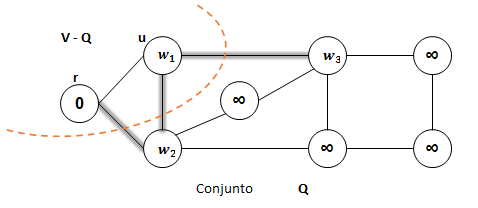
\includegraphics[width=0.6\textwidth]{q8-10.png}
\captionof{figure}{Exemplo de corte no grafo mostrando que o atributo $key[v] < \infty$ para os vértices adjacentes a $u$. As arestas sombreadas são aquelas atravessando o corte.}
\label{fig:8.10-1}
\end{center}